\section{Background}\label{sec:background}
\subsection{Machine Learning \& Artificial Neural Networks}\label{subsec:machine-learning-and-neural-networks}
Machine learning is a sub-field of artificial intelligence which "provides learning capability to computers
without being explicitly programmed"~\cite{Alzubi_2018}.
More specifically, machine learning allows computers to "learn" patterns and trends from existing data in order to make accurate predictions on new, unseen data.

Artificial neural networks (ANNs), meanwhile, are a type of machine learning model which draws inspiration from the human brain~\cite{Wang2003}.
These types of models feature "neurons" organized into densely connected layers.
Each connection between two neurons has an associated weight and bias, which determine how much the output from the source neuron affects the output of the destination neuron.
These values change as the model "learns" from existing data, causing the network's performance to gradually improve.
In addition to this, each neuron passes the combined input of all neurons in the previous layer through a non-linear activation function, which is what allows neural networks to effectively model any function possible~\cite{Wang2003}.

Although ANNs are no longer considered state-of-the-art, understanding the purposes of neurons, neuron connections, and activation functions remains useful, as these still form the building blocks of any neural network architecture.

\begin{figure}[h]
    \centering
    \captionsetup{justification=centering}
    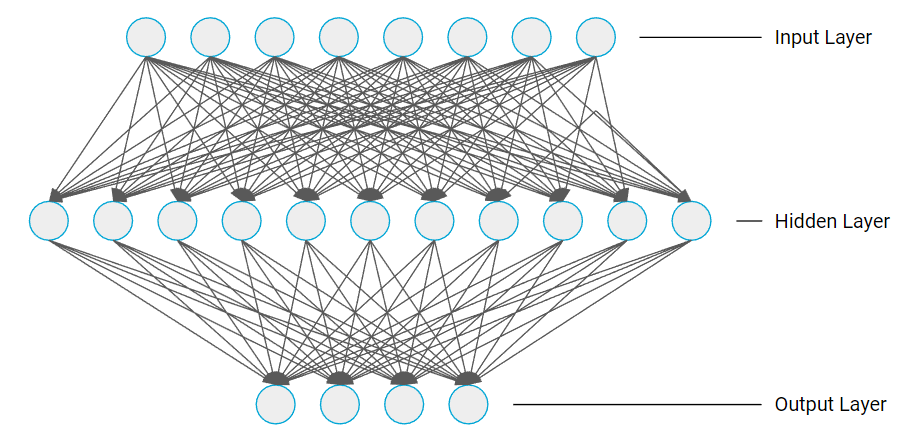
\includegraphics[width=\linewidth]{figures/ann}
    \caption{Visualization of a generic ANN with 8 input neurons and 4 output neurons, as well as a single hidden layer with 11 neurons.}
    \label{fig:ann}
\end{figure}

\subsection{Neural Networks on Embedded Hardware}\label{subsec:machine-learning-on-microcontrollers}
Machine learning, and specifically neural networks, have traditionally been restricted to the realms of high-performance and in turn, high power devices~\cite{8342164}.
Unfortunately, this means that it has been previously unfeasible to use these technologies with embedded hardware such as microcontrollers, as they lack the performance to run inference on neural networks locally, and the dedicated power to be able to transmit sensor data to a remote processor.

However, recent advances into machine learning model compression and optimization have changed this, allowing deep neural networks to be run on devices even powered by coin batteries.
The most prominent development in this field has been TensorFlow Lite for Microcontrollers, which is a Python framework specifically made for optimizing and running neural networks on microcontrollers~\cite{MLSYS2021_d2ddea18}.
The original Tensorflow has been an extremely popular machine learning framework for over a decade, but the extension to make it work effectively on microcontrollers has only been developed in recent years.

\subsection{Hand Gesture Data}\label{subsec:hand-gesture-data}
In this research, neural networks are used to detect gestures, but to do this, data from some sensor(s) must be fed into the network.

There are a variety of sensors which could be used to record hand gestures and provide this data.
One of these is an accelerometer attached to the user's wrist (typically from a smartwatch) to track the direction and acceleration of the their hand movements~\cite{4912759}.
Another option is using a depth/range camera to record the user's hand, which provides a huge amount of information but in turn requires a computationally intensive video processing pipeline to make sense of the data~\cite{article}.
Photodiodes can also be used, which are sensors that output a signal which increases with the amount of light that hits them.
This means they can effectively track shadows cast by the user's hand when some ambient light is present, therefore making it possible to recognize which gesture is being performed~\cite{8947919}.
This project uses photodiodes for their much lower monetary and computational cost compared to cameras as well as the fact that they don't require the user to wear a device on their wrists, unlike accelerometers.
